\documentclass[]{article}
\usepackage{lmodern}
\usepackage{amssymb,amsmath}
\usepackage{ifxetex,ifluatex}
\usepackage{fixltx2e} % provides \textsubscript
\ifnum 0\ifxetex 1\fi\ifluatex 1\fi=0 % if pdftex
  \usepackage[T1]{fontenc}
  \usepackage[utf8]{inputenc}
\else % if luatex or xelatex
  \ifxetex
    \usepackage{mathspec}
  \else
    \usepackage{fontspec}
  \fi
  \defaultfontfeatures{Ligatures=TeX,Scale=MatchLowercase}
\fi
% use upquote if available, for straight quotes in verbatim environments
\IfFileExists{upquote.sty}{\usepackage{upquote}}{}
% use microtype if available
\IfFileExists{microtype.sty}{%
\usepackage{microtype}
\UseMicrotypeSet[protrusion]{basicmath} % disable protrusion for tt fonts
}{}
\usepackage[margin=1in]{geometry}
\usepackage{hyperref}
\hypersetup{unicode=true,
            pdftitle={Baixando e analisando dados de alta frequência},
            pdfauthor={Lucca Simeoni Pavan  João Carlos de Carvalho},
            pdfborder={0 0 0},
            breaklinks=true}
\urlstyle{same}  % don't use monospace font for urls
\usepackage{color}
\usepackage{fancyvrb}
\newcommand{\VerbBar}{|}
\newcommand{\VERB}{\Verb[commandchars=\\\{\}]}
\DefineVerbatimEnvironment{Highlighting}{Verbatim}{commandchars=\\\{\}}
% Add ',fontsize=\small' for more characters per line
\usepackage{framed}
\definecolor{shadecolor}{RGB}{248,248,248}
\newenvironment{Shaded}{\begin{snugshade}}{\end{snugshade}}
\newcommand{\KeywordTok}[1]{\textcolor[rgb]{0.13,0.29,0.53}{\textbf{{#1}}}}
\newcommand{\DataTypeTok}[1]{\textcolor[rgb]{0.13,0.29,0.53}{{#1}}}
\newcommand{\DecValTok}[1]{\textcolor[rgb]{0.00,0.00,0.81}{{#1}}}
\newcommand{\BaseNTok}[1]{\textcolor[rgb]{0.00,0.00,0.81}{{#1}}}
\newcommand{\FloatTok}[1]{\textcolor[rgb]{0.00,0.00,0.81}{{#1}}}
\newcommand{\ConstantTok}[1]{\textcolor[rgb]{0.00,0.00,0.00}{{#1}}}
\newcommand{\CharTok}[1]{\textcolor[rgb]{0.31,0.60,0.02}{{#1}}}
\newcommand{\SpecialCharTok}[1]{\textcolor[rgb]{0.00,0.00,0.00}{{#1}}}
\newcommand{\StringTok}[1]{\textcolor[rgb]{0.31,0.60,0.02}{{#1}}}
\newcommand{\VerbatimStringTok}[1]{\textcolor[rgb]{0.31,0.60,0.02}{{#1}}}
\newcommand{\SpecialStringTok}[1]{\textcolor[rgb]{0.31,0.60,0.02}{{#1}}}
\newcommand{\ImportTok}[1]{{#1}}
\newcommand{\CommentTok}[1]{\textcolor[rgb]{0.56,0.35,0.01}{\textit{{#1}}}}
\newcommand{\DocumentationTok}[1]{\textcolor[rgb]{0.56,0.35,0.01}{\textbf{\textit{{#1}}}}}
\newcommand{\AnnotationTok}[1]{\textcolor[rgb]{0.56,0.35,0.01}{\textbf{\textit{{#1}}}}}
\newcommand{\CommentVarTok}[1]{\textcolor[rgb]{0.56,0.35,0.01}{\textbf{\textit{{#1}}}}}
\newcommand{\OtherTok}[1]{\textcolor[rgb]{0.56,0.35,0.01}{{#1}}}
\newcommand{\FunctionTok}[1]{\textcolor[rgb]{0.00,0.00,0.00}{{#1}}}
\newcommand{\VariableTok}[1]{\textcolor[rgb]{0.00,0.00,0.00}{{#1}}}
\newcommand{\ControlFlowTok}[1]{\textcolor[rgb]{0.13,0.29,0.53}{\textbf{{#1}}}}
\newcommand{\OperatorTok}[1]{\textcolor[rgb]{0.81,0.36,0.00}{\textbf{{#1}}}}
\newcommand{\BuiltInTok}[1]{{#1}}
\newcommand{\ExtensionTok}[1]{{#1}}
\newcommand{\PreprocessorTok}[1]{\textcolor[rgb]{0.56,0.35,0.01}{\textit{{#1}}}}
\newcommand{\AttributeTok}[1]{\textcolor[rgb]{0.77,0.63,0.00}{{#1}}}
\newcommand{\RegionMarkerTok}[1]{{#1}}
\newcommand{\InformationTok}[1]{\textcolor[rgb]{0.56,0.35,0.01}{\textbf{\textit{{#1}}}}}
\newcommand{\WarningTok}[1]{\textcolor[rgb]{0.56,0.35,0.01}{\textbf{\textit{{#1}}}}}
\newcommand{\AlertTok}[1]{\textcolor[rgb]{0.94,0.16,0.16}{{#1}}}
\newcommand{\ErrorTok}[1]{\textcolor[rgb]{0.64,0.00,0.00}{\textbf{{#1}}}}
\newcommand{\NormalTok}[1]{{#1}}
\usepackage{graphicx,grffile}
\makeatletter
\def\maxwidth{\ifdim\Gin@nat@width>\linewidth\linewidth\else\Gin@nat@width\fi}
\def\maxheight{\ifdim\Gin@nat@height>\textheight\textheight\else\Gin@nat@height\fi}
\makeatother
% Scale images if necessary, so that they will not overflow the page
% margins by default, and it is still possible to overwrite the defaults
% using explicit options in \includegraphics[width, height, ...]{}
\setkeys{Gin}{width=\maxwidth,height=\maxheight,keepaspectratio}
\IfFileExists{parskip.sty}{%
\usepackage{parskip}
}{% else
\setlength{\parindent}{0pt}
\setlength{\parskip}{6pt plus 2pt minus 1pt}
}
\setlength{\emergencystretch}{3em}  % prevent overfull lines
\providecommand{\tightlist}{%
  \setlength{\itemsep}{0pt}\setlength{\parskip}{0pt}}
\setcounter{secnumdepth}{5}
% Redefines (sub)paragraphs to behave more like sections
\ifx\paragraph\undefined\else
\let\oldparagraph\paragraph
\renewcommand{\paragraph}[1]{\oldparagraph{#1}\mbox{}}
\fi
\ifx\subparagraph\undefined\else
\let\oldsubparagraph\subparagraph
\renewcommand{\subparagraph}[1]{\oldsubparagraph{#1}\mbox{}}
\fi

%%% Use protect on footnotes to avoid problems with footnotes in titles
\let\rmarkdownfootnote\footnote%
\def\footnote{\protect\rmarkdownfootnote}

%%% Change title format to be more compact
\usepackage{titling}

% Create subtitle command for use in maketitle
\newcommand{\subtitle}[1]{
  \posttitle{
    \begin{center}\large#1\end{center}
    }
}

\setlength{\droptitle}{-2em}
  \title{Baixando e analisando dados de alta frequência}
  \pretitle{\vspace{\droptitle}\centering\huge}
  \posttitle{\par}
  \author{Lucca Simeoni Pavan \hspace{1cm} João Carlos de Carvalho}
  \preauthor{\centering\large\emph}
  \postauthor{\par}
  \predate{\centering\large\emph}
  \postdate{\par}
  \date{\today}

\setlength\parindent{24pt}
\usepackage[english, brazil]{babel}
\usepackage[utf8]{inputenc}
\usepackage{longtable}
\usepackage{booktabs}

\begin{document}
\maketitle

{
\setcounter{tocdepth}{2}
\tableofcontents
}
\begin{Shaded}
\begin{Highlighting}[]
\NormalTok{knitr::opts_chunk$}\KeywordTok{set}\NormalTok{(}\DataTypeTok{echo =} \OtherTok{TRUE}\NormalTok{, }\DataTypeTok{cache =} \OtherTok{FALSE}\NormalTok{, }\DataTypeTok{fig.height =} \DecValTok{4}\NormalTok{, }\DataTypeTok{warning =} \OtherTok{FALSE}\NormalTok{, }
    \DataTypeTok{message =} \OtherTok{FALSE}\NormalTok{, }\DataTypeTok{error =} \OtherTok{FALSE}\NormalTok{, }\DataTypeTok{tidy =} \OtherTok{TRUE}\NormalTok{, }\DataTypeTok{tidy.opts =} \KeywordTok{list}\NormalTok{(}\DataTypeTok{width.cutoff =} \DecValTok{70}\NormalTok{))}
\end{Highlighting}
\end{Shaded}

\section{Ranking de negociações}\label{ranking-de-negociacoes}

\begin{Shaded}
\begin{Highlighting}[]
\KeywordTok{library}\NormalTok{(GetHFData)}
\NormalTok{tickers_equity <-}\StringTok{ }\KeywordTok{ghfd_get_available_tickers_from_ftp}\NormalTok{(}\DataTypeTok{my.date =} \StringTok{"2016-10-30"}\NormalTok{, }
    \DataTypeTok{type.market =} \StringTok{"equity"}\NormalTok{, }\DataTypeTok{max.dl.tries =} \DecValTok{10}\NormalTok{)}
\end{Highlighting}
\end{Shaded}

\begin{verbatim}
## 
## Reading ftp contents for equity (attempt = 1|10) - Error in reading ftp contents. Trying again..
## Reading ftp contents for equity (attempt = 2|10) Attempt 1 - File exists, skipping dl
\end{verbatim}

\begin{Shaded}
\begin{Highlighting}[]
\KeywordTok{head}\NormalTok{(tickers_equity, }\DataTypeTok{n =} \DecValTok{10}\NormalTok{)}
\end{Highlighting}
\end{Shaded}

\begin{verbatim}
##    tickers n.trades                     f.name
## 1    PETR4    52393 ftp files/NEG_20161117.zip
## 2    JBSS3    45174 ftp files/NEG_20161117.zip
## 3    ITSA4    39200 ftp files/NEG_20161117.zip
## 4    ITUB4    30529 ftp files/NEG_20161117.zip
## 5    VALE5    30423 ftp files/NEG_20161117.zip
## 6    BVMF3    29099 ftp files/NEG_20161117.zip
## 7    BBDC4    26923 ftp files/NEG_20161117.zip
## 8    ABEV3    26786 ftp files/NEG_20161117.zip
## 9    BBAS3    26672 ftp files/NEG_20161117.zip
## 10   RUMO3    26274 ftp files/NEG_20161117.zip
\end{verbatim}

Criando um vetor com as 6 ações mais negociadas em 30/10/2016.

\begin{Shaded}
\begin{Highlighting}[]
\NormalTok{top_6 <-}\StringTok{ }\KeywordTok{c}\NormalTok{(}\KeywordTok{as.character}\NormalTok{(}\KeywordTok{head}\NormalTok{(tickers_equity$tickers)))}
\KeywordTok{print}\NormalTok{(top_6)}
\end{Highlighting}
\end{Shaded}

\begin{verbatim}
## [1] "PETR4" "JBSS3" "ITSA4" "ITUB4" "VALE5" "BVMF3"
\end{verbatim}

Baixando os dados

\begin{Shaded}
\begin{Highlighting}[]
\NormalTok{dados_top6 <-}\StringTok{ }\KeywordTok{ghfd_get_HF_data}\NormalTok{(top_6, }\DataTypeTok{type.market =} \StringTok{"equity"}\NormalTok{, }\DataTypeTok{first.date =} \KeywordTok{as.Date}\NormalTok{(}\StringTok{"2014-11-03"}\NormalTok{), }
    \DataTypeTok{last.date =} \KeywordTok{as.Date}\NormalTok{(}\StringTok{"2016-10-30"}\NormalTok{), }\DataTypeTok{first.time =} \StringTok{"9:00:00"}\NormalTok{, }\DataTypeTok{last.time =} \StringTok{"18:00:00"}\NormalTok{, }
    \DataTypeTok{type.output =} \StringTok{"agg"}\NormalTok{, }\DataTypeTok{agg.diff =} \StringTok{"1 hour"}\NormalTok{, }\DataTypeTok{dl.dir =} \StringTok{"ftp files"}\NormalTok{, }\DataTypeTok{max.dl.tries =} \DecValTok{10}\NormalTok{, }
    \DataTypeTok{clean.files =} \OtherTok{FALSE}\NormalTok{)}
\KeywordTok{save}\NormalTok{(dados_top6, }\DataTypeTok{file =} \StringTok{"dados_top6.Rda"}\NormalTok{)}
\KeywordTok{head}\NormalTok{(dados_top6, }\DataTypeTok{n =} \DecValTok{6}\NormalTok{)}
\end{Highlighting}
\end{Shaded}

\begin{Shaded}
\begin{Highlighting}[]
\KeywordTok{load}\NormalTok{(}\StringTok{"dados_top6.Rda"}\NormalTok{)}
\KeywordTok{dim}\NormalTok{(dados_top6)}
\end{Highlighting}
\end{Shaded}

\begin{verbatim}
## [1] 22667    13
\end{verbatim}

\begin{Shaded}
\begin{Highlighting}[]
\KeywordTok{str}\NormalTok{(dados_top6)}
\end{Highlighting}
\end{Shaded}

\begin{verbatim}
## 'data.frame':    22667 obs. of  13 variables:
##  $ InstrumentSymbol: chr  "ABEV3" "ABEV3" "ABEV3" "ABEV3" ...
##  $ SessionDate     : Date, format: "2014-11-03" "2014-11-03" ...
##  $ TradeDateTime   : POSIXct, format: "2014-11-03 10:00:00" "2014-11-03 11:00:00" ...
##  $ n.trades        : int  1607 2055 3417 3686 3978 4707 5168 250 1602 1203 ...
##  $ last.price      : num  16.1 16.1 16.2 16.1 16.1 ...
##  $ weighted.price  : num  16.1 16.1 16.2 16.2 16.1 ...
##  $ period.ret      : num  -0.00864 0.00124 0.0056 -0.00124 -0.00372 ...
##  $ period.ret.volat: num  0.000325 0.000324 0.000278 0.000235 0.000263 ...
##  $ sum.qtd         : num  824900 926700 1408500 1034900 1141100 ...
##  $ sum.vol         : num  13291157 14907444 22757436 16729199 18362060 ...
##  $ n.buys          : int  579 1113 1888 2265 1972 1878 2309 23 659 526 ...
##  $ n.sells         : int  1028 942 1529 1421 2006 2829 2859 227 943 677 ...
##  $ Tradetime       : chr  "10:00:00" "11:00:00" "12:00:00" "13:00:00" ...
\end{verbatim}

Agora irei criar um banco de dados para cada ação e depois obter os log
retornos.

\begin{Shaded}
\begin{Highlighting}[]
\KeywordTok{library}\NormalTok{(dplyr)}
\NormalTok{dados_ITSA4 <-}\StringTok{ }\KeywordTok{filter}\NormalTok{(dados_top6, InstrumentSymbol ==}\StringTok{ "ITSA4"}\NormalTok{) %>%}\StringTok{ }
\StringTok{    }\KeywordTok{select}\NormalTok{(SessionDate, weighted.price) %>%}\StringTok{ }\KeywordTok{mutate}\NormalTok{(}\DataTypeTok{log_retorno =} \KeywordTok{log}\NormalTok{(weighted.price) -}\StringTok{ }
\StringTok{    }\KeywordTok{lag}\NormalTok{(}\KeywordTok{log}\NormalTok{(weighted.price)))}
\NormalTok{dados_PETR4 <-}\StringTok{ }\KeywordTok{filter}\NormalTok{(dados_top6, InstrumentSymbol ==}\StringTok{ "PETR4"}\NormalTok{) %>%}\StringTok{ }
\StringTok{    }\KeywordTok{select}\NormalTok{(SessionDate, weighted.price) %>%}\StringTok{ }\KeywordTok{mutate}\NormalTok{(}\DataTypeTok{log_retorno =} \KeywordTok{log}\NormalTok{(weighted.price) -}\StringTok{ }
\StringTok{    }\KeywordTok{lag}\NormalTok{(}\KeywordTok{log}\NormalTok{(weighted.price)))}
\NormalTok{dados_ITUB4 <-}\StringTok{ }\KeywordTok{filter}\NormalTok{(dados_top6, InstrumentSymbol ==}\StringTok{ "ITUB4"}\NormalTok{) %>%}\StringTok{ }
\StringTok{    }\KeywordTok{select}\NormalTok{(SessionDate, weighted.price) %>%}\StringTok{ }\KeywordTok{mutate}\NormalTok{(}\DataTypeTok{log_retorno =} \KeywordTok{log}\NormalTok{(weighted.price) -}\StringTok{ }
\StringTok{    }\KeywordTok{lag}\NormalTok{(}\KeywordTok{log}\NormalTok{(weighted.price)))}
\NormalTok{dados_BBDC4 <-}\StringTok{ }\KeywordTok{filter}\NormalTok{(dados_top6, InstrumentSymbol ==}\StringTok{ "BBDC4"}\NormalTok{) %>%}\StringTok{ }
\StringTok{    }\KeywordTok{select}\NormalTok{(SessionDate, weighted.price) %>%}\StringTok{ }\KeywordTok{mutate}\NormalTok{(}\DataTypeTok{log_retorno =} \KeywordTok{log}\NormalTok{(weighted.price) -}\StringTok{ }
\StringTok{    }\KeywordTok{lag}\NormalTok{(}\KeywordTok{log}\NormalTok{(weighted.price)))}
\NormalTok{dados_ABEV3 <-}\StringTok{ }\KeywordTok{filter}\NormalTok{(dados_top6, InstrumentSymbol ==}\StringTok{ "ABEV3"}\NormalTok{) %>%}\StringTok{ }
\StringTok{    }\KeywordTok{select}\NormalTok{(SessionDate, weighted.price) %>%}\StringTok{ }\KeywordTok{mutate}\NormalTok{(}\DataTypeTok{log_retorno =} \KeywordTok{log}\NormalTok{(weighted.price) -}\StringTok{ }
\StringTok{    }\KeywordTok{lag}\NormalTok{(}\KeywordTok{log}\NormalTok{(weighted.price))) %>%}\StringTok{ }\KeywordTok{mutate}\NormalTok{(}\DataTypeTok{log_retorno =} \KeywordTok{log}\NormalTok{(weighted.price) -}\StringTok{ }
\StringTok{    }\KeywordTok{lag}\NormalTok{(}\KeywordTok{log}\NormalTok{(weighted.price)))}
\NormalTok{dados_BBSE3 <-}\StringTok{ }\KeywordTok{filter}\NormalTok{(dados_top6, InstrumentSymbol ==}\StringTok{ "BBSE3"}\NormalTok{) %>%}\StringTok{ }
\StringTok{    }\KeywordTok{select}\NormalTok{(SessionDate, weighted.price) %>%}\StringTok{ }\KeywordTok{mutate}\NormalTok{(}\DataTypeTok{log_retorno =} \KeywordTok{log}\NormalTok{(weighted.price) -}\StringTok{ }
\StringTok{    }\KeywordTok{lag}\NormalTok{(}\KeywordTok{log}\NormalTok{(weighted.price)))}
\end{Highlighting}
\end{Shaded}

Removendo \texttt{NA}s.

\begin{Shaded}
\begin{Highlighting}[]
\NormalTok{dados_BBSE3 <-}\StringTok{ }\NormalTok{dados_BBSE3[}\DecValTok{2}\NormalTok{:}\DecValTok{3778}\NormalTok{, ]}
\NormalTok{dados_ABEV3 <-}\StringTok{ }\NormalTok{dados_ABEV3[}\DecValTok{2}\NormalTok{:}\DecValTok{3778}\NormalTok{, ]}
\NormalTok{dados_BBDC4 <-}\StringTok{ }\NormalTok{dados_BBDC4[}\DecValTok{2}\NormalTok{:}\DecValTok{3778}\NormalTok{, ]}
\NormalTok{dados_ITUB4 <-}\StringTok{ }\NormalTok{dados_ITUB4[}\DecValTok{2}\NormalTok{:}\DecValTok{3778}\NormalTok{, ]}
\NormalTok{dados_PETR4 <-}\StringTok{ }\NormalTok{dados_PETR4[}\DecValTok{2}\NormalTok{:}\DecValTok{3777}\NormalTok{, ]}
\NormalTok{dados_ITSA4 <-}\StringTok{ }\NormalTok{dados_ITSA4[}\DecValTok{2}\NormalTok{:}\DecValTok{3778}\NormalTok{, ]}
\end{Highlighting}
\end{Shaded}

\section{Descrição dos Dados}\label{descricao-dos-dados}

Representação dos preços.

\begin{Shaded}
\begin{Highlighting}[]
\NormalTok{matriz_preco <-}\StringTok{ }\KeywordTok{data.frame}\NormalTok{(}\DataTypeTok{ITSA4 =} \NormalTok{(dados_ITSA4$weighted.price), }\DataTypeTok{ITUB4 =} \NormalTok{(dados_ITUB4$weighted.price), }
    \DataTypeTok{BBDC4 =} \NormalTok{(dados_BBDC4$weighted.price), }\DataTypeTok{ABEV3 =} \NormalTok{(dados_ABEV3$weighted.price), }
    \DataTypeTok{BBSE3 =} \NormalTok{(dados_BBSE3$weighted.price))}
\KeywordTok{library}\NormalTok{(BMR)}
\KeywordTok{gtsplot}\NormalTok{(matriz_preco)}
\end{Highlighting}
\end{Shaded}

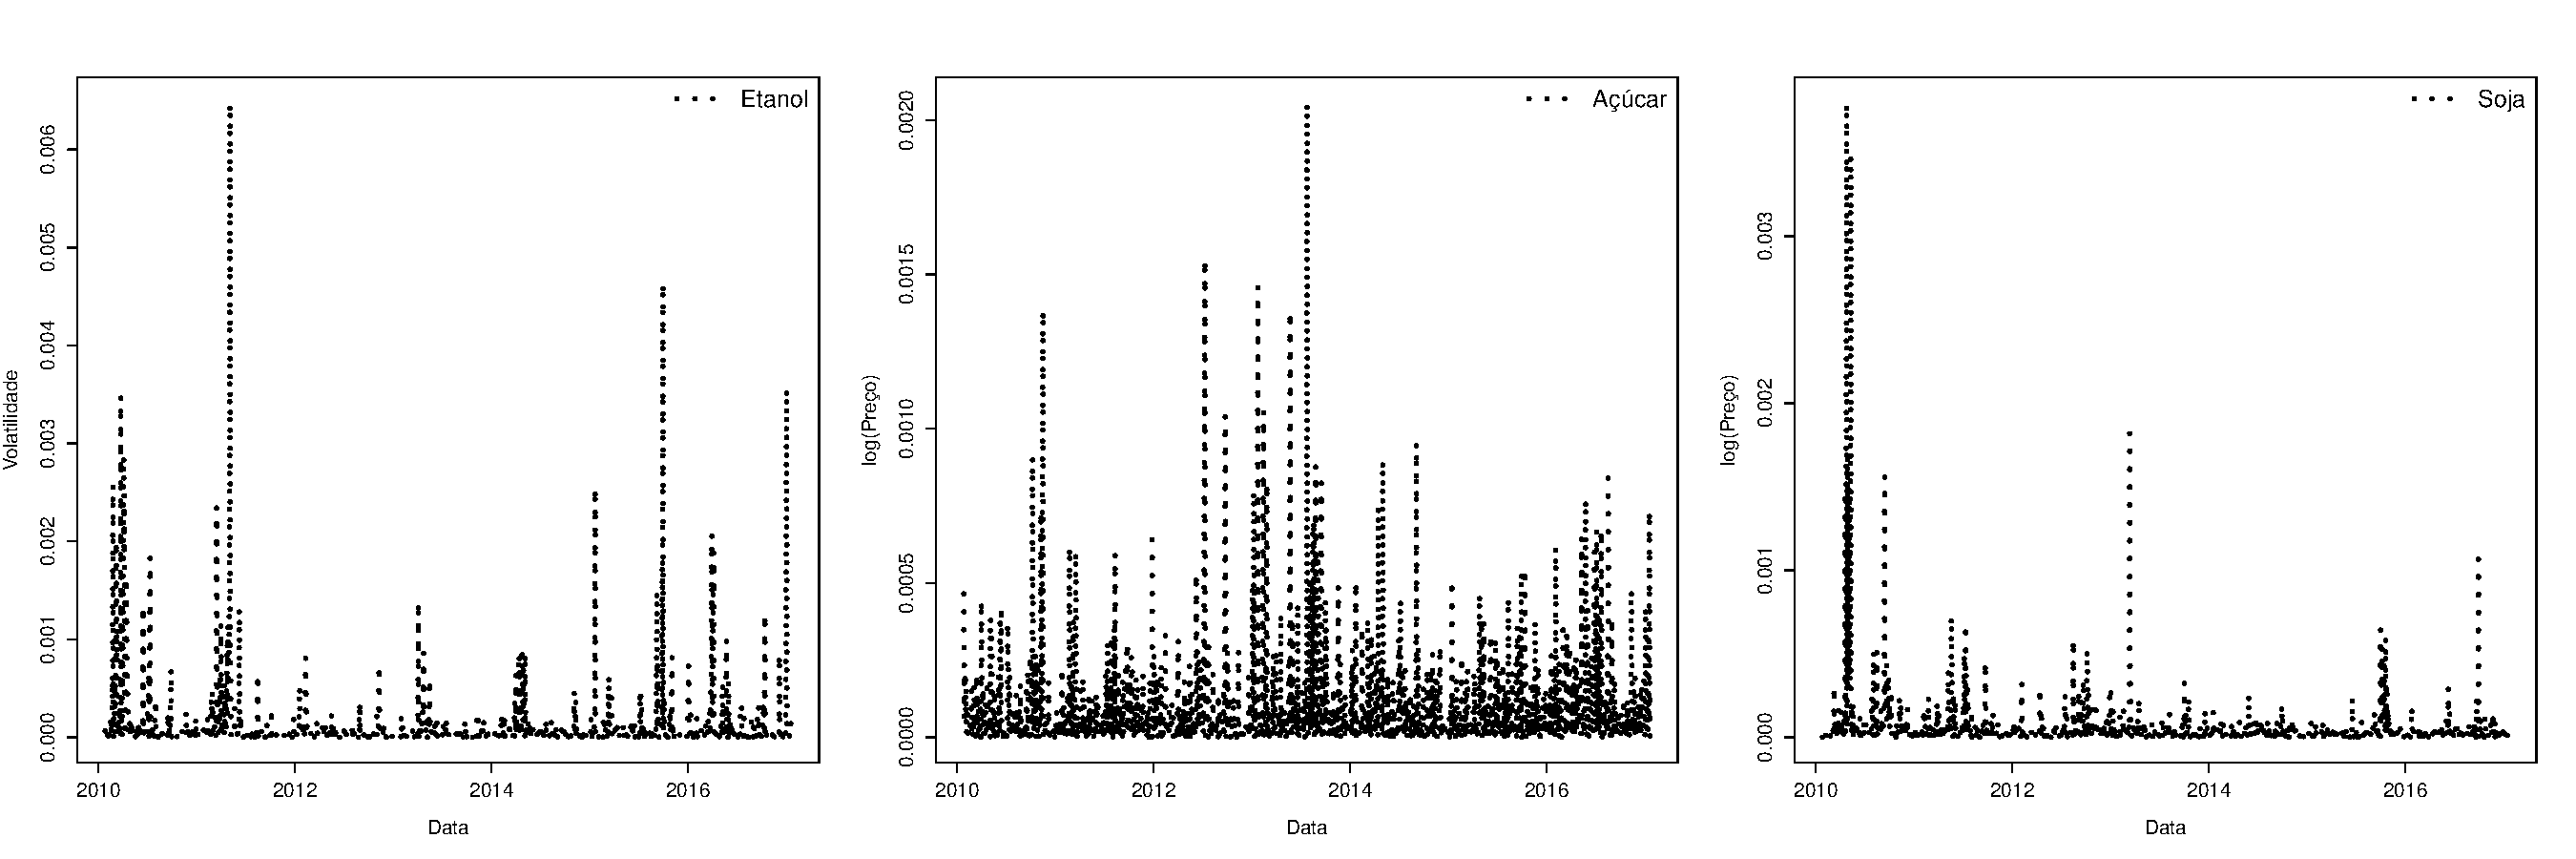
\includegraphics{Baixando_analisando_dados_af_files/figure-latex/unnamed-chunk-5-1.pdf}

\begin{Shaded}
\begin{Highlighting}[]
\KeywordTok{summary}\NormalTok{(matriz_preco)}
\end{Highlighting}
\end{Shaded}

\begin{verbatim}
##      ITSA4            ITUB4           BBDC4           ABEV3      
##  Min.   : 6.268   Min.   :22.93   Min.   :16.98   Min.   :15.16  
##  1st Qu.: 7.429   1st Qu.:28.40   1st Qu.:23.33   1st Qu.:18.15  
##  Median : 8.353   Median :32.66   Median :27.61   Median :18.79  
##  Mean   : 8.390   Mean   :31.81   Mean   :27.62   Mean   :18.52  
##  3rd Qu.: 9.339   3rd Qu.:35.25   3rd Qu.:31.15   3rd Qu.:19.26  
##  Max.   :10.897   Max.   :40.00   Max.   :41.22   Max.   :20.40  
##      BBSE3      
##  Min.   :21.12  
##  1st Qu.:27.69  
##  Median :29.80  
##  Mean   :29.71  
##  3rd Qu.:31.99  
##  Max.   :37.50
\end{verbatim}

\begin{Shaded}
\begin{Highlighting}[]
\KeywordTok{cov}\NormalTok{(matriz_preco)}
\end{Highlighting}
\end{Shaded}

\begin{verbatim}
##            ITSA4      ITUB4     BBDC4      ABEV3      BBSE3
## ITSA4  1.2634470  4.1766452  5.701124 -0.2390199  3.0699712
## ITUB4  4.1766452 16.6835114 19.773773 -0.1993035 10.9002367
## BBDC4  5.7011238 19.7737733 30.416024 -2.0025240 12.7153579
## ABEV3 -0.2390199 -0.1993035 -2.002524  1.1330387  0.3676802
## BBSE3  3.0699712 10.9002367 12.715358  0.3676802 10.7679356
\end{verbatim}

Criando matriz de log dos preços.

\begin{Shaded}
\begin{Highlighting}[]
\NormalTok{matriz_logpreco <-}\StringTok{ }\KeywordTok{data.frame}\NormalTok{(}\DataTypeTok{ITSA4 =} \KeywordTok{log}\NormalTok{(dados_ITSA4$weighted.price), }
    \DataTypeTok{ITUB4 =} \KeywordTok{log}\NormalTok{(dados_ITUB4$weighted.price), }\DataTypeTok{BBDC4 =} \KeywordTok{log}\NormalTok{(dados_BBDC4$weighted.price), }
    \DataTypeTok{ABEV3 =} \KeywordTok{log}\NormalTok{(dados_ABEV3$weighted.price), }\DataTypeTok{BBSE3 =} \KeywordTok{log}\NormalTok{(dados_BBSE3$weighted.price))}
\KeywordTok{library}\NormalTok{(BMR)}
\KeywordTok{gtsplot}\NormalTok{(matriz_logpreco)}
\end{Highlighting}
\end{Shaded}

\includegraphics{Baixando_analisando_dados_af_files/figure-latex/unnamed-chunk-6-1.pdf}

\begin{Shaded}
\begin{Highlighting}[]
\KeywordTok{summary}\NormalTok{(matriz_logpreco)}
\end{Highlighting}
\end{Shaded}

\begin{verbatim}
##      ITSA4           ITUB4           BBDC4           ABEV3      
##  Min.   :1.835   Min.   :3.132   Min.   :2.832   Min.   :2.718  
##  1st Qu.:2.005   1st Qu.:3.346   1st Qu.:3.150   1st Qu.:2.898  
##  Median :2.123   Median :3.486   Median :3.318   Median :2.933  
##  Mean   :2.118   Mean   :3.451   Mean   :3.298   Mean   :2.917  
##  3rd Qu.:2.234   3rd Qu.:3.562   3rd Qu.:3.439   3rd Qu.:2.958  
##  Max.   :2.388   Max.   :3.689   Max.   :3.719   Max.   :3.016  
##      BBSE3      
##  Min.   :3.050  
##  1st Qu.:3.321  
##  Median :3.395  
##  Mean   :3.385  
##  3rd Qu.:3.465  
##  Max.   :3.624
\end{verbatim}

\begin{Shaded}
\begin{Highlighting}[]
\KeywordTok{cov}\NormalTok{(matriz_logpreco)}
\end{Highlighting}
\end{Shaded}

\begin{verbatim}
##             ITSA4         ITUB4        BBDC4         ABEV3        BBSE3
## ITSA4  0.01787547  0.0162354679  0.025154358 -0.0014471303 0.0128461741
## ITUB4  0.01623547  0.0175130525  0.024189973 -0.0002988126 0.0123718427
## BBDC4  0.02515436  0.0241899729  0.040909538 -0.0032696184 0.0173792039
## ABEV3 -0.00144713 -0.0002988126 -0.003269618  0.0035513228 0.0007159475
## BBSE3  0.01284617  0.0123718427  0.017379204  0.0007159475 0.0127852450
\end{verbatim}

Criando matriz com os dados log retorno.

\begin{Shaded}
\begin{Highlighting}[]
\NormalTok{matriz_logrtn <-}\StringTok{ }\KeywordTok{data.frame}\NormalTok{(}\DataTypeTok{ITSA4 =} \NormalTok{dados_ITSA4$log_retorno, }\DataTypeTok{ITUB4 =} \NormalTok{dados_ITUB4$log_retorno, }
    \DataTypeTok{BBDC4 =} \NormalTok{dados_BBDC4$log_retorno, }\DataTypeTok{ABEV3 =} \NormalTok{dados_ABEV3$log_retorno, }\DataTypeTok{BBSE3 =} \NormalTok{dados_BBSE3$log_retorno)}
\KeywordTok{summary}\NormalTok{(matriz_logrtn)}
\end{Highlighting}
\end{Shaded}

\begin{verbatim}
##      ITSA4                ITUB4                BBDC4           
##  Min.   :-1.079e-01   Min.   :-9.911e-02   Min.   :-1.976e-01  
##  1st Qu.:-3.412e-03   1st Qu.:-3.276e-03   1st Qu.:-3.698e-03  
##  Median :-1.467e-04   Median :-5.178e-05   Median :-3.910e-06  
##  Mean   :-4.198e-05   Mean   :-5.640e-06   Mean   :-5.718e-05  
##  3rd Qu.: 3.154e-03   3rd Qu.: 3.205e-03   3rd Qu.: 3.599e-03  
##  Max.   : 7.451e-02   Max.   : 8.019e-02   Max.   : 7.990e-02  
##      ABEV3                BBSE3           
##  Min.   :-4.289e-02   Min.   :-6.050e-02  
##  1st Qu.:-2.287e-03   1st Qu.:-3.531e-03  
##  Median : 7.486e-05   Median : 1.017e-05  
##  Mean   : 5.483e-05   Mean   :-2.386e-05  
##  3rd Qu.: 2.359e-03   3rd Qu.: 3.362e-03  
##  Max.   : 2.241e-02   Max.   : 8.743e-02
\end{verbatim}

\begin{Shaded}
\begin{Highlighting}[]
\KeywordTok{cov}\NormalTok{(matriz_logrtn)}
\end{Highlighting}
\end{Shaded}

\begin{verbatim}
##              ITSA4        ITUB4        BBDC4        ABEV3        BBSE3
## ITSA4 5.167608e-05 4.335244e-05 4.281033e-05 1.524743e-05 2.995500e-05
## ITUB4 4.335244e-05 5.104148e-05 4.627070e-05 1.615010e-05 3.064427e-05
## BBDC4 4.281033e-05 4.627070e-05 6.736253e-05 1.655762e-05 3.067263e-05
## ABEV3 1.524743e-05 1.615010e-05 1.655762e-05 2.114459e-05 1.369144e-05
## BBSE3 2.995500e-05 3.064427e-05 3.067263e-05 1.369144e-05 5.436357e-05
\end{verbatim}

\begin{Shaded}
\begin{Highlighting}[]
\KeywordTok{cor}\NormalTok{(matriz_logrtn)}
\end{Highlighting}
\end{Shaded}

\begin{verbatim}
##           ITSA4     ITUB4     BBDC4     ABEV3     BBSE3
## ITSA4 1.0000000 0.8441257 0.7255955 0.4612668 0.5651589
## ITUB4 0.8441257 1.0000000 0.7891058 0.4916024 0.5817463
## BBDC4 0.7255955 0.7891058 1.0000000 0.4387216 0.5068598
## ABEV3 0.4612668 0.4916024 0.4387216 1.0000000 0.4038272
## BBSE3 0.5651589 0.5817463 0.5068598 0.4038272 1.0000000
\end{verbatim}

\begin{Shaded}
\begin{Highlighting}[]
\KeywordTok{library}\NormalTok{(BMR)}
\KeywordTok{gtsplot}\NormalTok{(matriz_logrtn)}
\end{Highlighting}
\end{Shaded}

\includegraphics{Baixando_analisando_dados_af_files/figure-latex/unnamed-chunk-8-1.pdf}

\begin{Shaded}
\begin{Highlighting}[]
\KeywordTok{head}\NormalTok{(matriz_logrtn)}
\end{Highlighting}
\end{Shaded}

\begin{verbatim}
##           ITSA4         ITUB4        BBDC4         ABEV3        BBSE3
## 1 -0.0079058649 -0.0057653310 -0.004521064 -0.0016150278 -0.010986101
## 2  0.0050112343  0.0045462710 -0.002177734  0.0043904510  0.008955299
## 3 -0.0030588852 -0.0059963761 -0.001079848  0.0004751700 -0.004649955
## 4 -0.0036985681 -0.0022077264 -0.006330370 -0.0045601580 -0.009555026
## 5  0.0019715511  0.0028860314  0.003117587 -0.0008106029  0.013210150
## 6  0.0002158613 -0.0003814315 -0.004567171 -0.0029404438 -0.006192878
\end{verbatim}

\section{Testes de Estacionariedade}\label{testes-de-estacionariedade}

\begin{Shaded}
\begin{Highlighting}[]
\KeywordTok{library}\NormalTok{(BMR)}
\KeywordTok{library}\NormalTok{(knitr)}
\NormalTok{stat1 <-}\StringTok{ }\KeywordTok{stationarity}\NormalTok{(matriz_preco, }\DecValTok{4}\NormalTok{, }\DecValTok{8}\NormalTok{)}
\end{Highlighting}
\end{Shaded}

\begin{Shaded}
\begin{Highlighting}[]
\KeywordTok{kable}\NormalTok{(stat1$KPSS, }\DataTypeTok{caption =} \StringTok{"Teste KPSS (preço)"}\NormalTok{, }\DataTypeTok{format =} \StringTok{"latex"}\NormalTok{, }\DataTypeTok{booktabs =} \OtherTok{TRUE}\NormalTok{, }
    \DataTypeTok{longtable =} \OtherTok{TRUE}\NormalTok{, }\DataTypeTok{digits =} \DecValTok{2}\NormalTok{)}
\end{Highlighting}
\end{Shaded}

\begin{longtable}[t]{lrrrrrrrrr}
\caption{\label{tab:unnamed-chunk-10}Teste KPSS (preço)}\\
\toprule
  & ITSA4 & ITUB4 & BBDC4 & ABEV3 & BBSE3 & 1 Pct & 2.5 Pct & 5 Pct & 10 Pct\\
\midrule
Time Trend: & 11.18 & 12.47 & 15.64 & 7.35 & 6.16 & 0.22 & 0.18 & 0.15 & 0.12\\
No Trend: & 39.72 & 20.86 & 37.71 & 22.77 & 25.09 & 0.74 & 0.57 & 0.46 & 0.35\\
\bottomrule
\end{longtable}

\begin{Shaded}
\begin{Highlighting}[]
\KeywordTok{kable}\NormalTok{(stat1$ADF, }\DataTypeTok{caption =} \StringTok{"Teste ADF (preço)"}\NormalTok{, }\DataTypeTok{format =} \StringTok{"latex"}\NormalTok{, }\DataTypeTok{booktabs =} \OtherTok{TRUE}\NormalTok{, }
    \DataTypeTok{longtable =} \OtherTok{TRUE}\NormalTok{, }\DataTypeTok{digits =} \DecValTok{2}\NormalTok{)}
\end{Highlighting}
\end{Shaded}

\begin{longtable}[t]{lrrrrrrrrr}
\caption{\label{tab:unnamed-chunk-10}Teste ADF (preço)}\\
\toprule
  & ITSA4 & ITUB4 & BBDC4 & ABEV3 & BBSE3 & 1 Pct & 2.5 Pct & 5 Pct & 10 Pct\\
\midrule
Time Trend: & -2.09 & -1.73 & -1.40 & -3.10 & -2.46 & -3.96 & -3.66 & -3.41 & -3.12\\
Constant: & -1.98 & -1.94 & -1.85 & -2.81 & -2.34 & -3.43 & -3.12 & -2.86 & -2.57\\
Neither: & -0.61 & -0.30 & -0.80 & 0.57 & -0.45 & -2.58 & -2.23 & -1.95 & -1.62\\
\bottomrule
\end{longtable}

\begin{Shaded}
\begin{Highlighting}[]
\KeywordTok{kable}\NormalTok{(stat1$ADFLags, }\DataTypeTok{caption =} \StringTok{"Defagens do teste ADF (preço)"}\NormalTok{, }\DataTypeTok{format =} \StringTok{"latex"}\NormalTok{, }
    \DataTypeTok{booktabs =} \OtherTok{TRUE}\NormalTok{, }\DataTypeTok{longtable =} \OtherTok{TRUE}\NormalTok{, }\DataTypeTok{digits =} \DecValTok{2}\NormalTok{)}
\end{Highlighting}
\end{Shaded}

\begin{longtable}[t]{lrrr}
\caption{\label{tab:unnamed-chunk-10}Defagens do teste ADF (preço)}\\
\toprule
  & Trend Model & Drift Model & None\\
\midrule
ITSA4 & 1 & 1 & 1\\
ITUB4 & 1 & 1 & 1\\
BBDC4 & 1 & 1 & 1\\
ABEV3 & 3 & 3 & 3\\
BBSE3 & 1 & 1 & 1\\
\bottomrule
\end{longtable}

\begin{Shaded}
\begin{Highlighting}[]
\NormalTok{stat2 <-}\StringTok{ }\KeywordTok{stationarity}\NormalTok{(matriz_logpreco, }\DecValTok{4}\NormalTok{, }\DecValTok{8}\NormalTok{)}
\end{Highlighting}
\end{Shaded}

\begin{Shaded}
\begin{Highlighting}[]
\KeywordTok{kable}\NormalTok{(stat2$KPSS, }\DataTypeTok{caption =} \StringTok{"Teste KPSS (log preço)"}\NormalTok{, }\DataTypeTok{format =} \StringTok{"latex"}\NormalTok{, }
    \DataTypeTok{booktabs =} \OtherTok{TRUE}\NormalTok{, }\DataTypeTok{longtable =} \OtherTok{TRUE}\NormalTok{, }\DataTypeTok{digits =} \DecValTok{2}\NormalTok{)}
\end{Highlighting}
\end{Shaded}

\begin{longtable}[t]{lrrrrrrrrr}
\caption{\label{tab:unnamed-chunk-11}Teste KPSS (log preço)}\\
\toprule
  & ITSA4 & ITUB4 & BBDC4 & ABEV3 & BBSE3 & 1 Pct & 2.5 Pct & 5 Pct & 10 Pct\\
\midrule
Time Trend: & 11.09 & 12.39 & 14.92 & 7.46 & 6.27 & 0.22 & 0.18 & 0.15 & 0.12\\
No Trend: & 38.14 & 20.20 & 34.35 & 23.00 & 24.10 & 0.74 & 0.57 & 0.46 & 0.35\\
\bottomrule
\end{longtable}

\begin{Shaded}
\begin{Highlighting}[]
\KeywordTok{kable}\NormalTok{(stat2$ADF, }\DataTypeTok{caption =} \StringTok{"Teste ADF (log preço)"}\NormalTok{, }\DataTypeTok{format =} \StringTok{"latex"}\NormalTok{, }\DataTypeTok{booktabs =} \OtherTok{TRUE}\NormalTok{, }
    \DataTypeTok{longtable =} \OtherTok{TRUE}\NormalTok{, }\DataTypeTok{digits =} \DecValTok{2}\NormalTok{)}
\end{Highlighting}
\end{Shaded}

\begin{longtable}[t]{lrrrrrrrrr}
\caption{\label{tab:unnamed-chunk-11}Teste ADF (log preço)}\\
\toprule
  & ITSA4 & ITUB4 & BBDC4 & ABEV3 & BBSE3 & 1 Pct & 2.5 Pct & 5 Pct & 10 Pct\\
\midrule
Time Trend: & -2.03 & -1.71 & -1.27 & -3.06 & -2.44 & -3.96 & -3.66 & -3.41 & -3.12\\
Constant: & -1.97 & -1.91 & -1.73 & -2.80 & -2.34 & -3.43 & -3.12 & -2.86 & -2.57\\
Neither: & -0.45 & -0.12 & -0.49 & 0.69 & -0.25 & -2.58 & -2.23 & -1.95 & -1.62\\
\bottomrule
\end{longtable}

\begin{Shaded}
\begin{Highlighting}[]
\KeywordTok{kable}\NormalTok{(stat2$ADFLags, }\DataTypeTok{caption =} \StringTok{"Defagens do teste ADF (log preço)"}\NormalTok{, }\DataTypeTok{format =} \StringTok{"latex"}\NormalTok{, }
    \DataTypeTok{booktabs =} \OtherTok{TRUE}\NormalTok{, }\DataTypeTok{longtable =} \OtherTok{TRUE}\NormalTok{, }\DataTypeTok{digits =} \DecValTok{2}\NormalTok{)}
\end{Highlighting}
\end{Shaded}

\begin{longtable}[t]{lrrr}
\caption{\label{tab:unnamed-chunk-11}Defagens do teste ADF (log preço)}\\
\toprule
  & Trend Model & Drift Model & None\\
\midrule
ITSA4 & 1 & 1 & 1\\
ITUB4 & 1 & 1 & 1\\
BBDC4 & 1 & 1 & 1\\
ABEV3 & 3 & 3 & 3\\
BBSE3 & 1 & 1 & 1\\
\bottomrule
\end{longtable}

\begin{Shaded}
\begin{Highlighting}[]
\NormalTok{stat3 <-}\StringTok{ }\KeywordTok{stationarity}\NormalTok{(matriz_logrtn, }\DecValTok{4}\NormalTok{, }\DecValTok{8}\NormalTok{)}
\end{Highlighting}
\end{Shaded}

\begin{Shaded}
\begin{Highlighting}[]
\KeywordTok{kable}\NormalTok{(stat3$KPSS, }\DataTypeTok{caption =} \StringTok{"Teste KPSS (log retorno)"}\NormalTok{, }\DataTypeTok{format =} \StringTok{"latex"}\NormalTok{, }
    \DataTypeTok{booktabs =} \OtherTok{TRUE}\NormalTok{, }\DataTypeTok{longtable =} \OtherTok{TRUE}\NormalTok{, }\DataTypeTok{digits =} \DecValTok{2}\NormalTok{)}
\end{Highlighting}
\end{Shaded}

\begin{longtable}[t]{lrrrrrrrrr}
\caption{\label{tab:unnamed-chunk-12}Teste KPSS (log retorno)}\\
\toprule
  & ITSA4 & ITUB4 & BBDC4 & ABEV3 & BBSE3 & 1 Pct & 2.5 Pct & 5 Pct & 10 Pct\\
\midrule
Time Trend: & 0.04 & 0.04 & 0.05 & 0.03 & 0.04 & 0.22 & 0.18 & 0.15 & 0.12\\
No Trend: & 0.09 & 0.14 & 0.23 & 0.05 & 0.06 & 0.74 & 0.57 & 0.46 & 0.35\\
\bottomrule
\end{longtable}

\begin{Shaded}
\begin{Highlighting}[]
\KeywordTok{kable}\NormalTok{(stat3$ADF, }\DataTypeTok{caption =} \StringTok{"Teste ADF (log retorno)"}\NormalTok{, }\DataTypeTok{format =} \StringTok{"latex"}\NormalTok{, }
    \DataTypeTok{booktabs =} \OtherTok{TRUE}\NormalTok{, }\DataTypeTok{longtable =} \OtherTok{TRUE}\NormalTok{, }\DataTypeTok{digits =} \DecValTok{2}\NormalTok{)}
\end{Highlighting}
\end{Shaded}

\begin{longtable}[t]{lrrrrrrrrr}
\caption{\label{tab:unnamed-chunk-12}Teste ADF (log retorno)}\\
\toprule
  & ITSA4 & ITUB4 & BBDC4 & ABEV3 & BBSE3 & 1 Pct & 2.5 Pct & 5 Pct & 10 Pct\\
\midrule
Time Trend: & -41.94 & -40.48 & -40.65 & -37.49 & -42.03 & -3.96 & -3.66 & -3.41 & -3.12\\
Constant: & -41.94 & -40.47 & -40.63 & -37.49 & -42.03 & -3.43 & -3.12 & -2.86 & -2.57\\
Neither: & -41.94 & -40.48 & -40.63 & -37.49 & -42.04 & -2.58 & -2.23 & -1.95 & -1.62\\
\bottomrule
\end{longtable}

\begin{Shaded}
\begin{Highlighting}[]
\KeywordTok{kable}\NormalTok{(stat3$ADFLags, }\DataTypeTok{caption =} \StringTok{"Defagens do teste ADF (log retorno)"}\NormalTok{, }\DataTypeTok{format =} \StringTok{"latex"}\NormalTok{, }
    \DataTypeTok{booktabs =} \OtherTok{TRUE}\NormalTok{, }\DataTypeTok{longtable =} \OtherTok{TRUE}\NormalTok{, }\DataTypeTok{digits =} \DecValTok{2}\NormalTok{)}
\end{Highlighting}
\end{Shaded}

\begin{longtable}[t]{lrrr}
\caption{\label{tab:unnamed-chunk-12}Defagens do teste ADF (log retorno)}\\
\toprule
  & Trend Model & Drift Model & None\\
\midrule
ITSA4 & 1 & 1 & 1\\
ITUB4 & 1 & 1 & 1\\
BBDC4 & 1 & 1 & 1\\
ABEV3 & 2 & 2 & 2\\
BBSE3 & 1 & 1 & 1\\
\bottomrule
\end{longtable}

\begin{Shaded}
\begin{Highlighting}[]
\KeywordTok{library}\NormalTok{(BMR)}
\KeywordTok{gacf}\NormalTok{(matriz_logrtn)}
\end{Highlighting}
\end{Shaded}

\includegraphics{Baixando_analisando_dados_af_files/figure-latex/unnamed-chunk-13-1.pdf}

\begin{Shaded}
\begin{Highlighting}[]
\KeywordTok{gpacf}\NormalTok{(matriz_logrtn)}
\end{Highlighting}
\end{Shaded}

\includegraphics{Baixando_analisando_dados_af_files/figure-latex/unnamed-chunk-13-2.pdf}

\begin{Shaded}
\begin{Highlighting}[]
\KeywordTok{save}\NormalTok{(matriz_preco, }\DataTypeTok{file =} \StringTok{"matriz_preco.Rda"}\NormalTok{)}
\KeywordTok{save}\NormalTok{(matriz_logrtn, }\DataTypeTok{file =} \StringTok{"matriz_logrtn.Rda"}\NormalTok{)}
\end{Highlighting}
\end{Shaded}

\begin{Shaded}
\begin{Highlighting}[]
\KeywordTok{acf}\NormalTok{(matriz_logrtn)}
\end{Highlighting}
\end{Shaded}

\includegraphics{Baixando_analisando_dados_af_files/figure-latex/unnamed-chunk-14-1.pdf}

\begin{Shaded}
\begin{Highlighting}[]
\KeywordTok{acf}\NormalTok{(matriz_logrtn, }\DataTypeTok{type =} \StringTok{"partial"}\NormalTok{)}
\end{Highlighting}
\end{Shaded}

\includegraphics{Baixando_analisando_dados_af_files/figure-latex/unnamed-chunk-14-2.pdf}

\begin{Shaded}
\begin{Highlighting}[]
\KeywordTok{library}\NormalTok{(MVN)}
\KeywordTok{uniPlot}\NormalTok{(matriz_logrtn, }\DataTypeTok{type =} \StringTok{"qqplot"}\NormalTok{)}
\KeywordTok{uniPlot}\NormalTok{(matriz_logrtn, }\DataTypeTok{type =} \StringTok{"box"}\NormalTok{)}
\end{Highlighting}
\end{Shaded}

\includegraphics{Baixando_analisando_dados_af_files/figure-latex/unnamed-chunk-15-1.pdf}

\begin{Shaded}
\begin{Highlighting}[]
\KeywordTok{uniPlot}\NormalTok{(matriz_logrtn, }\DataTypeTok{type =} \StringTok{"scatter"}\NormalTok{)}
\end{Highlighting}
\end{Shaded}

\includegraphics{Baixando_analisando_dados_af_files/figure-latex/unnamed-chunk-15-2.pdf}

\begin{Shaded}
\begin{Highlighting}[]
\KeywordTok{uniPlot}\NormalTok{(matriz_logrtn, }\DataTypeTok{type =} \StringTok{"histogram"}\NormalTok{)}
\end{Highlighting}
\end{Shaded}

\includegraphics{Baixando_analisando_dados_af_files/figure-latex/unnamed-chunk-16-1.pdf}

\begin{Shaded}
\begin{Highlighting}[]
\KeywordTok{library}\NormalTok{(MVN)}
\KeywordTok{library}\NormalTok{(fBasics)}
\KeywordTok{uniNorm}\NormalTok{(matriz_logrtn)}
\end{Highlighting}
\end{Shaded}

\begin{verbatim}
## $`Descriptive Statistics`
##          n Mean Std.Dev Median    Min   Max   25th  75th   Skew Kurtosis
## ITSA4 3777    0   0.007      0 -0.108 0.075 -0.003 0.003 -1.225   34.177
## ITUB4 3777    0   0.007      0 -0.099 0.080 -0.003 0.003 -0.135   22.259
## BBDC4 3777    0   0.008      0 -0.198 0.080 -0.004 0.004 -3.842  101.520
## ABEV3 3777    0   0.005      0 -0.043 0.022 -0.002 0.002 -0.383    5.151
## BBSE3 3777    0   0.007      0 -0.060 0.087 -0.004 0.003  0.369   11.993
## 
## $`Shapiro-Wilk's Normality Test`
##    Variable Statistic   p-value Normality
## 1   ITSA4      0.8502         0    NO    
## 2   ITUB4      0.8742         0    NO    
## 3   BBDC4      0.7937         0    NO    
## 4   ABEV3      0.9517         0    NO    
## 5   BBSE3      0.9191         0    NO
\end{verbatim}

\begin{Shaded}
\begin{Highlighting}[]
\KeywordTok{jarqueberaTest}\NormalTok{(matriz_logrtn$ITSA4)}
\end{Highlighting}
\end{Shaded}

\begin{verbatim}
## 
## Title:
##  Jarque - Bera Normalality Test
## 
## Test Results:
##   STATISTIC:
##     X-squared: 184985.3846
##   P VALUE:
##     Asymptotic p Value: < 2.2e-16 
## 
## Description:
##  Thu Dec 08 15:46:56 2016 by user: Lucca
\end{verbatim}

\begin{Shaded}
\begin{Highlighting}[]
\KeywordTok{jarqueberaTest}\NormalTok{(matriz_logrtn$ITUB4)}
\end{Highlighting}
\end{Shaded}

\begin{verbatim}
## 
## Title:
##  Jarque - Bera Normalality Test
## 
## Test Results:
##   STATISTIC:
##     X-squared: 78079.208
##   P VALUE:
##     Asymptotic p Value: < 2.2e-16 
## 
## Description:
##  Thu Dec 08 15:46:56 2016 by user: Lucca
\end{verbatim}

\begin{Shaded}
\begin{Highlighting}[]
\KeywordTok{jarqueberaTest}\NormalTok{(matriz_logrtn$BBDC4)}
\end{Highlighting}
\end{Shaded}

\begin{verbatim}
## 
## Title:
##  Jarque - Bera Normalality Test
## 
## Test Results:
##   STATISTIC:
##     X-squared: 1633035.358
##   P VALUE:
##     Asymptotic p Value: < 2.2e-16 
## 
## Description:
##  Thu Dec 08 15:46:56 2016 by user: Lucca
\end{verbatim}

\begin{Shaded}
\begin{Highlighting}[]
\KeywordTok{jarqueberaTest}\NormalTok{(matriz_logrtn$ABEV3)}
\end{Highlighting}
\end{Shaded}

\begin{verbatim}
## 
## Title:
##  Jarque - Bera Normalality Test
## 
## Test Results:
##   STATISTIC:
##     X-squared: 4274.4093
##   P VALUE:
##     Asymptotic p Value: < 2.2e-16 
## 
## Description:
##  Thu Dec 08 15:46:56 2016 by user: Lucca
\end{verbatim}

\begin{Shaded}
\begin{Highlighting}[]
\KeywordTok{jarqueberaTest}\NormalTok{(matriz_logrtn$BBSE3)}
\end{Highlighting}
\end{Shaded}

\begin{verbatim}
## 
## Title:
##  Jarque - Bera Normalality Test
## 
## Test Results:
##   STATISTIC:
##     X-squared: 22752.1698
##   P VALUE:
##     Asymptotic p Value: < 2.2e-16 
## 
## Description:
##  Thu Dec 08 15:46:56 2016 by user: Lucca
\end{verbatim}

\begin{Shaded}
\begin{Highlighting}[]
\KeywordTok{library}\NormalTok{(MTS)}
\KeywordTok{mq}\NormalTok{(matriz_logrtn, }\DataTypeTok{lag =} \DecValTok{10}\NormalTok{)}
\end{Highlighting}
\end{Shaded}

\begin{verbatim}
## Ljung-Box Statistics:  
##         m       Q(m)     df    p-value
##  [1,]     1       156      25        0
##  [2,]     2       202      50        0
##  [3,]     3       252      75        0
##  [4,]     4       265     100        0
##  [5,]     5       298     125        0
##  [6,]     6       318     150        0
##  [7,]     7       349     175        0
##  [8,]     8       408     200        0
##  [9,]     9       442     225        0
## [10,]    10       465     250        0
\end{verbatim}

\includegraphics{Baixando_analisando_dados_af_files/figure-latex/unnamed-chunk-18-1.pdf}


\end{document}
